\documentclass[25pt,margin=1in,innermargin=-4.5in,blockverticalspace=-0.25in]{tikzposter}
\geometry{paperwidth=42in,paperheight=30in}
\usepackage[utf8]{inputenc}
\usepackage{csquotes}
% \usepackage[estonian]{babel}
\usepackage{amsmath}
\usepackage{amsfonts}
\usepackage{amsthm}
\usepackage{amssymb}
\usepackage{mathrsfs}
\usepackage{graphicx}
\usepackage{subcaption}
\usepackage{adjustbox}
\usepackage{enumitem}
\usepackage{xcolor}
\usepackage[backend=bibtex,style=numeric,sorting=none,maxbibnames=3,minbibnames=1,
giveninits=true,doi=false,url=false,isbn=false,eprint=false]{biblatex}
\renewcommand*{\bibfont}{\normalsize}
\setlength{\bibitemsep}{0.3\baselineskip}

\usepackage{unitartu-theme}
\usepackage{etoolbox}
\AtBeginEnvironment{tikzfigure}{\captionsetup{type=figure}}
\DeclareMathOperator*{\argmin}{arg\,min}



\usepackage{mwe} % for placeholder images
\usepackage{lipsum}
\setlength\headheight{26pt} %% just to make warning go away. Adjust the value after looking into the warning.
% \rhead{{\color{blue}\rule{1cm}{1cm}}}


\addbibresource{ref.bib}

% set theme parameters
\tikzposterlatexaffectionproofoff
\usetheme{UniTartuTheme}
\usecolorstyle{UniTartuStyle}

\usepackage[scaled]{helvet}
\renewcommand\familydefault{\sfdefault} 
\renewcommand{\vec}[1]{\bm{#1}}
\newcommand{\Tr}{\text{Tr}}
\newcommand{\comment}[1]{}
\usepackage[T1]{fontenc}
\usepackage{enumitem} 

\title{CantataS: a \textcolor{MainBlue}{C}ommunity-\textcolor{MainBlue}{a}ware age\textcolor{MainBlue}{nt}-b\textcolor{MainBlue}{a}sed ci\textcolor{MainBlue}{ta}tion \textcolor{MainBlue}{S}imulator}
\author{Hemank Kohli, Tandy Warnow, and George Chacko}
% and \textbf{Jane Smith}\textsuperscript{2} % Add 2nd author

\institute{Siebel School of Computing and Data Science \\ University of Illinois at Urbana-Champaign, Urbana, IL}
% \titlegraphic{\vspace{-0.1}\raisebox{0.1}{
% \includegraphics[width=0.15\linewidth]{nips_logo.png}}}
% \titlegraphic{\hspace{10.5}\vspace{0.2}\raisebox{10}{
% \includegraphics[width=0.15\linewidth]{nips_logo.png}}}
% \usepackage{tikz}
% \titlegraphic{ \begin{tikzpicture}[overlay,remember picture]
% \node[left=-0.2cm]{
%     \includegraphics[width=0.15\linewidth]{nips_logo.png}
% }
% \end{tikzpicture}
% }
%\titlegraphic
\includegraphics[width=0.15\linewidth]{figures/illinois_cs_logo.png}}
%\titlegraphic{
\includegraphics[width=0.15\linewidth]{figures/illinois_cs_logo.png}}
%\titlegraphic{
\includegraphics[width=0.08\linewidth]{figures/siebel.png}}
%\titlegraphic{
\includegraphics[width=0.06\linewidth]{figures/logo_cna2026_textorange.png}}
%\titlegraphic{\includegraphics[width=0.15\linewidth]{nips_logo.png}}

\titlegraphic{%
  
\includegraphics[height=4cm]{figures/siebel.png}%
  \hspace{1.5cm}%
  
\includegraphics[height=4cm]{figures/logo_cna2026_textorange.png}%
}

% begin document
\begin{document}
\maketitle
\centering
\begin{columns}
    \column{0.32}
    
    \block{Motivation}{
         \begin{itemize}[itemsep=1.3em]
           \item Understanding how, why, and what researchers cite is of broad interest
           \item Observations in the modern scientific enterprise are incommensurable with earlier studies
           \item Simulations under agent-based models complement social theory and mathematical models
         \end{itemize}  
         \vspace{5mm}
    }
    
     \block{Background}{
         \begin{itemize}[itemsep=1.3em]
           \item Building upon prior work, we have developed a series of idealized agent-based models of citation \cite{Chacko2026,Park2026a,Park2026b,Park2026c} 
           \item These generative models return a citation network with nodes as articles and edges as citations
           \item CantataS adds community-awareness as a feature in addition to preferential attachment, fitness, recency, and author reputation
         \end{itemize}  
         \vspace{5mm}   
    }
    
    \block{Methods}{
         \begin{itemize}
            \item \begin{tikzfigure}[] 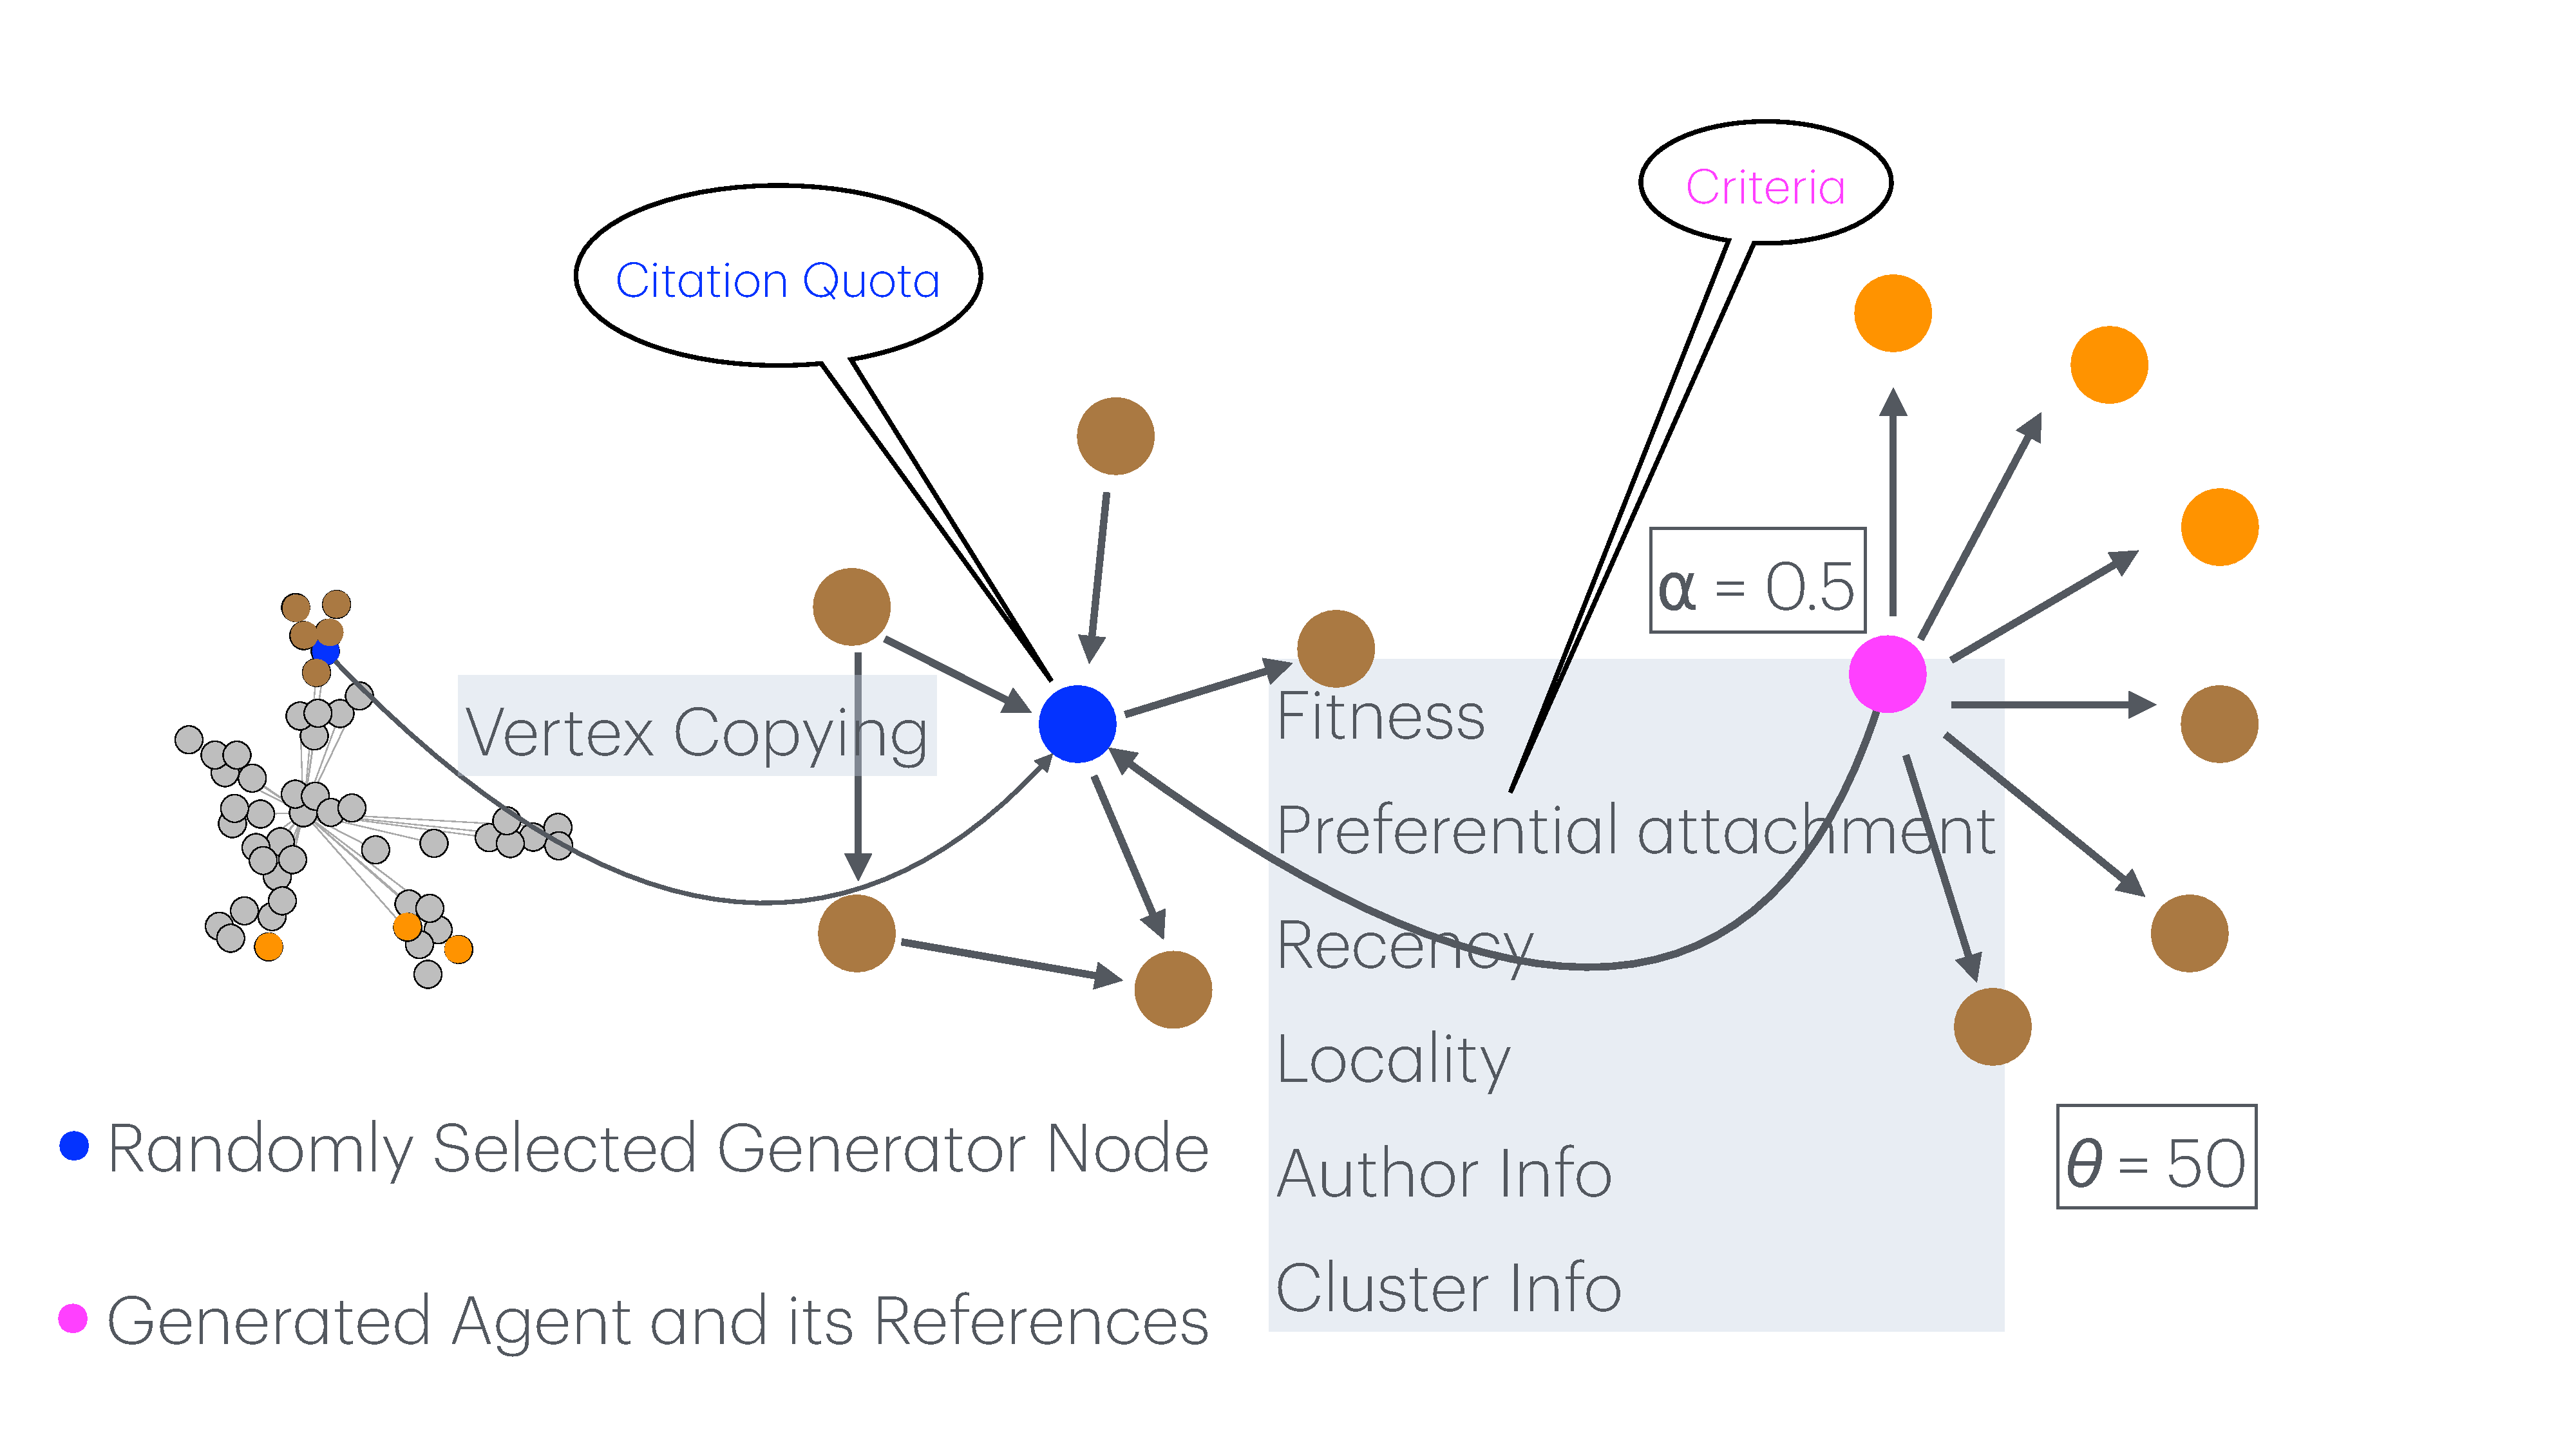
\includegraphics[width=0.95\linewidth]{figures/model.pdf} \end{tikzfigure} 
             \item b1
             \item b2
             \item b3
         \end{itemize}  
         \vspace{5mm}
    }
    \column{0.32}
    
    \block{Results}{
    \textbf{Limitations in prior work}
    \begin{itemize}
    \item b1
    \item b2
    \end{itemize} 
    
    \textbf{Our goals}
    \begin{itemize}
    \item Leverage invariant learning in causal effect estimation 
    \item Capture \textbf{non-linear} patterns in the data using an autoencoder framework
    \item Use latent-variable modeling that can be robust even with the existence of confounding variables and \textbf{covariate shifts} within control units
    \end{itemize} }
    \column{0.32}
    
    \block{Discussion}{
    \begin{itemize}
        \item We compared AE with state-of-the-art methods on CMAP dataset, which contains measurements of gene expression for more than 1 million samples.
        \item We measured accuracy in terms of root mean square error (RMSE), mean absolute error (MAE), and cosine similarity, which is an alignment measure. 
        \item The training and evaluation are done in a leave-one-out manner. The boxplots show error (with mean and standard deviation) across 519 samples.
       % \begin{tikzfigure}[] \includegraphics[width=0.58\linewidth]{figures/rmse_boxplot_all.png} \end{tikzfigure}
        
    \end{itemize} 
    }
    \block{}{
    \item \textbf{Observation:} The current AE framework outperforms \textbf{5 out of 6} baselines in terms of cosine similarity, and \textbf{4 out of 6} baselines in terms of RMSE.
    %\begin{tikzfigure}[] 
    %\includegraphics[width=0.58\linewidth]{figures/cosine_boxplot_all.png}
    %\end{tikzfigure}
    }
    w
    
    \block{References}{
        \vspace{-1em}
        \begin{normalsize}
        \printbibliography[heading=none]
        \end{normalsize}
    }
\end{columns}
\end{document}